\documentclass[times,onecolumn]{scrartcl} 
\usepackage{geometry}              
\usepackage{multirow}
\usepackage{graphicx}
\usepackage{amssymb}
\usepackage{amsmath}
\usepackage{times}
\usepackage{lineno}
\usepackage{color}
\renewcommand{\baselinestretch}{1.2}
\newcommand{\arne}[1]{\textcolor{red}{#1}}
\newcommand{\cha}[1]{\textcolor{blue}{#1}}
\newcommand{\leftsub}[2]{{\vphantom{#2}}_{#1}{#2}}



\begin{document}
\linenumbers

\title{Supplementary material: \\
Population dynamics of mutualisms}

\author{
Chaitanya S. Gokhale 
}

\maketitle

\section*{Interspecies Evolutionary Dynamics}

Traditional coevolutionary models consider interspecific dependence only \cite{roughgarden:TPB:1976,roughgarden:book:1983}.
Depicting the interaction between the two species as a multiplayer game \cite{gokhale:PNAS:2010}.
Assume Species $1$ is playing a $d_1^{inter}$ player game.
Hence we need to pick $d_1^{inter}-1$ individuals from Species $2$ for the interactions.
Similarly for Species $2$ playing a $d_2^{inter}$ player game means we pick $d_2^{inter}-1$ players from Species $1$.
Since in our case each the interactions between the Species are mutualistic and each Species consists of two types of individuals ``Generous" and ``Selfish", the following Snowdrift game is an appropriate representation of the interactions.
%This is because we have neglected intraspecific interactions as mentioned earlier.

%For different types of interactions between species differrent models need to be defined \cite{poulin:JTB:1995,doebeli:PNAS:1998,noe:book:2001,johnstone:ECL:2002,bergstrom:PNAS:2003,hoeksema:AmNat:2003,akcay:PRSB:2007,bshary:Nature:2008}.




\subsection*{The snowdrift game}
\label{appA}
\subsubsection*{Two player setting}
%So far, we have described general games within and between species, now we turn to a particular game which of interest to us when considering mutualism.
Two drivers are stuck in a snowdrift.
They must shovel away the snow (paying the cost $c$) to reach home (benefit $b$) but there are three possible outcomes to this scenario.
One of the driver shovels while the other stays warm in the care ($b-c$ and $b$), both the drivers share the workload and shovel away the snow ($b-c/2$ and $b-c/2$) or none of them gets out of the care and they both remain stuck ($0$ and $0$).

Putting this game in perspective of the two species (i.e. the two drivers represent the two different species) we get the matrix,\\
%
\begin{equation}\label{}
\begin{array}{cccc}
& & \multicolumn{2}{c}{\text{Species 2}}\\
\hline\hline
&	&	G_2		&	S_2	\\
\hline
 \multirow{2}{*}{Species 1} & G_1 	& b-c/2 &	b-c \\
&	S_1	&  b & 0 \\
 \hline\hline
\end{array}
\hspace{1cm}
\begin{array}{cccc}
& & \multicolumn{2}{c}{\text{Species 1}}\\
\hline\hline
&	&	G_1		&	S_1	\\
\hline
 \multirow{2}{*}{Species 2} & G_2 	& b-c/2 &	b-c \\
&	S_2	& b & 0 \nonumber \\
 \hline\hline
\end{array}
\end{equation}
%
where strategy $G$ stands for being \textit{``Generous"} and shoveling the snow while $S$ stands for being \textit{``Selfish"} and just sitting in the car.
For $b=2$ and $c=1$ we recover the matrix used in \cite{bergstrom:PNAS:2003}.

For the snowdrift game in a single population there exists a single, stable internal equilibrium.
Hence the population will evolve to a polymorphism which is a combination of \textit{``Generous"} and \textit{``Selfish"} individuals.
But in a two species system, this stable equilibrium turns into a saddle point, a small deviation from this fixed point can lead the system to one of the stable fixed point where one of the species is completely \textit{``Generous"} 
and the other one is completely \textit{``Selfish"}.

\subsection*{Multiplayer setting}
\label{appB}

Following Souza et al. \cite{souza:JTB:2009},  
a multiplayer snowdrift game can be described by the payoff entries
\begin{eqnarray}
\Pi_{G_1} (k)  &=& \begin{cases} b-\frac{c}{k} & \textrm{if } k \geq M \\  -\frac{c}{M} & \textrm{if } k < M \end{cases}
\\
\Pi_{S_1} (k)  &=& \begin{cases} b & \textrm{if } k \geq M \\ 0 & \textrm{if } k < M. \end{cases}
\end{eqnarray}
%
The selfish players get the benefit $b$ if the number of generous individuals in both species combined, $k$, is greater than or equal to the threshold $M$.
For the generous individuals, their effort is subtracted from the payoffs.
The effort is shared if the quorum size is met ($\frac{c}{M}$), but is in vain for $k<M$.
For two player games we had $k=1$ but multiplayer games provide the possibility of exploring this threshold aspect of collective action games.
From these payoff entries we need to calculate the average fitnesses.
For simplicity we just illustrate the fitnesses of the strategies in Species $1$.
For a $d_1^{inter}$ player game for Species $1$ we need to pick $d_1^{inter}-1$ other individuals from Species $2$.
Assuming random sampling the composition of the formed groups is given by a binomial distribution.
Summing over all possible compositions of groups we arrive at  the average fitnesses of the two strategies in species $1$,
%
\begin{align}
f^{inter}_{G_1} (y) &= \sum_{k=0}^{d_1^{inter} -1} \binom{d_1^{inter} -1}{k}y^k (1-y)^{d_1^{inter} -1-k} \Pi_{G_1}(k+1) \\
f^{inter}_{S_1} (y) &= \sum_{k=0}^{d_1^{inter} -1} \binom{d_1^{inter} -1}{k}y^k (1-y)^{d_1^{inter} -1-k} \Pi_{S_1}(k).
\label{interfiteqs}
\end{align}
%


\section*{Intraspecies Evolutionary Dynamics}
\label{appB}

For elucidating the intraspecies dynamics we will focus on Species $1$ as the analysis is analogous for Species $2$.
Withing species dynamics can in principle be completely different from the between species interactions. 
We can have a multistrategy multiplayer game within a Species but to keep things simple we assume a two strategy multiplayer game.
The partitioning of the individuals into two strategies follows the same partitioning as in the inter species interactions as of ``Generous" and ``Selfish". 
However we can relabel them as ``Cooperators" and ``Defector" for the sake of the interactions structure which we will be making use of.
Note that the ``Generous" in the interspecies interactions need not always be the ``Cooperators" for the within species interaction but again for the sake of simplicity we will assume it  to be so.

\subsection*{Synergy/Discounting Framework}
We model the within species interactions by making use of a general framework of costs and non-linear benefits \cite{eshel:AmNat:1988,hauert:JTB:2006a} which can potentially encompass all different types of social interaction structures qualitatively.
For Species $1$ the frequency of cooperators is just $x$ and the defectors is $1-x$, the same as the ``Generous" and ``Selfish".
The ``Cooperators" and ``Defectors" in Species $1$ play a $d_1^{intra}$ player game.
Thus the fitnesses of cooperators and defectors are defined as \cite{hauert:JTB:2006a},
%
\begin{align}
	f^{intra}_{G_1} (x) &= \sum_{k=0}^{d_1^{intra} -1} \binom{d_1^{intra} -1}{k}x^k (1-x)^{d_1^{intra} -1-k} \Gamma_{G_1}(k+1) \\
	f^{intra}_{S_1} (x) &= \sum_{k=0}^{d_1 -1} \binom{d_1^{intra} -1}{k}x^k (1-x)^{d_1^{intra} -1-k} \Gamma_{S_1}(k).
\label{intrafiteqs}
\end{align}
%
where the payoffs are given by,
\begin{align}
	\Gamma_{S_1} (k) = \frac{\tilde{b}}{d_1^{intra}} \sum_{i=0}^{k-1} \omega^i \\
	\Gamma_{G_1} (k) = \Gamma_{S_1} (k) - \tilde{c}.
\label{eqintragamepayoffs}
\end{align}
%
Thus the defectors get a fraction of the benefit which is scaled by the factor $\omega$, which determines if the benefits are linearly accumulating ($\omega=1$) for increasing number of cooperators, synergistically enhanced ($\omega>1$) or saturating ($\omega<1$).
Note that the costs and benefits in the within species game need not be (and naturally so) the same as in between species ($b\neq \tilde{b}$ and $c \neq \tilde{c}$).


\section*{Combined Evolutionary Dynamics}

The average payoffs are then just assumed to be a linear combination of the interspecies and intraspecies interactions where the parameter $p$ determines the strength of each of the interactions such that,
%
\begin{align}
	f_{G_1} (x,y) &= p f^{inter}_{G_1} (y) + (1-p) f^{intra}_{G_1} (x) \\
	f_{S_1} (x,y) &= p f^{inter}_{S_1} (y) + (1-p) f^{intra}_{S_1} (x)
\label{fiteqs}
\end{align}
%
Following the same procedure for the two strategies in species $2$ leads to the average fitness
%
\begin{align}
\bar{f}_1 (x,y) &= x f_{G_1} (x,y)+(1-x) f_ {S_1}(x,y)\\
\bar{f}_2 (x,y) &= y f_{G_2} (x,y)+(1-y) f_{S_2}(x,y).
\label{avgfiteqs}
\end{align}
%
The time evolution of the ``Generous" types in both the species will give us the complete dynamics of the system.
However since the two interaction species are by definition different organisms, they can have different rates of evolution.
Thus if species 1 evolves at the rate $r_x$ while species 2 at rate $r_y$ then we have,
\begin{align}
\dot{x} &= r_x x \left(f_{G_1}(x,y) -  \bar{f}_1(x,y) \right) \nonumber \\
\dot{y} &= r_y y \left(f_{G_2}(x,y) -  \bar{f}_2(x,y) \right).
\label{eq:repeqs}
\end{align}


\begin{figure*}[h]
\begin{center}
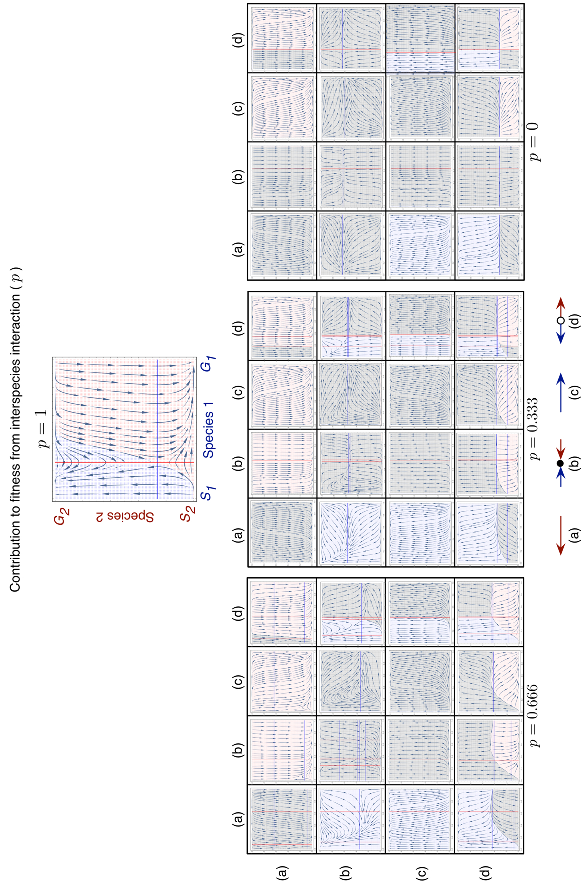
\includegraphics[width=\columnwidth]{../Figures/Dynamicsacrossp_reduced.pdf}
\caption{
$d_1^{inter} = d_2^{inter} = 5$, $b = 2$, $r_x = r_y/8$, $M_1 = M_2 = 1$ and $c=1$ for the interspecies game. As for the intraspecies games (a), (b), (c) and (d) the exact same parameter values as in \cite{hauert:JTB:2006a}.
}
\end{center}
\end{figure*}


\cha{\section*{Asymmetries}}

\cha{This between and within species model is a powerful way of introducing a lot of variability into the dynamics,
\begin{align}
	d_1 &\neq d_2 \\
	d^{inter} &\neq d^{intra} \\
	M_1 &\neq M_2 \\
	b &\neq \tilde{b} \\
	c &\neq \tilde{c} \\
	r_x &\neq r_y \\
	&\vdots
\end{align}
and various combinations of these. We should justify why we don't do this here and why we do vary the ones that we do.}


%\subsection{Dynamics in asymmetric conditions}
%
%%We have addressed two kinds of asymmetries in the game, the number of player and the thresholds in the two species.
%%We denote the number of players for species $1$ and species $2$ as $d_1$ and $d_2$, respectively, as in Fig.\ \ref{fig:counter}.
%%That is if species $2$ is playing a $d_2$ player game it means that one player from species $2$ interacts with $d_2-1$ players of species $1$.
%%For an asymmetry in the thresholds we use the two parameters $M_1\geq1$ and $M_2\geq1$ for the two species, respectively.
%
%For asymmetric bimatrix games, there is a difference in the dynamics between the standard replicator dynamics and the 
%alternative dynamics put forward by Maynard-Smith \cite{maynard-smith:1982to}.
%For this dynamics, the average fitness of each species appears as a denominator,
%\begin{align}
%\dot{x} &= r_x x \left(f_{G_1}(y) -  \bar{f}_1(x,y) \right)/\bar{f}_1(x,y) \nonumber \\
%\dot{y} &= r_y y \left(f_{G_2}(x) -  \bar{f}_2(x,y) \right)/\bar{f}_2(x,y).
%\label{eq:repeqs}
%\end{align}
%In our asymmetric bimatrix game, the fixed point stability is affected by the choice of the dynamics, in contrast to the case of symmetric games. 
%%In Fig.\ \ref{fig:thresholdsmodrep}, we illustrate that the dynamics is different between the usual replicator dynamics and Eqs. \ref{eq:repeqs}
%
%For $d_1=d_2 \geq 5$, the exact coordinates of the fixed point must be computed numerically \cite{abel:AO:1824,stewart:book:2004}.


\section*{Population dynamics}

For brevity we begin with the description of population dynamics in Species 1.
The two types in Species 1, ``Generous" and ``Selfish" need not sum up to $1$ i.e. the population may not always be at its carrying capacity.
Hence if the empty space in the niche occupied by Species $1$ is $z_1$, then we have $x_1 + x_2 + z_1 = $ where $x_1$ and $x_2$ are the densities of ``Generous" and ``Selfish" types.
The population dynamics then is dictated by,
%
\begin{align}
	\dot{x_1} &= r_x x_1 (z_1 f_{G_1} - e_1) \\
	\dot{x_2} &= r_x x_2 (z_1 f_{S_1} - e_1) \\
	\dot{z_1} &= - \dot{x_1} - \dot{x_2}
\end{align}
%
and for species 2
\begin{align}
	\dot{y_1} &= r_y y_1 (z_2 f_{G_2} - e_2) \\
	\dot{y_2} &= r_y y_2 (z_2 f_{S_2} - e_2) \\
	\dot{y_1} &= - \dot{y_1} - \dot{y_2}
\end{align}
%
We have $e_1$ and $e_2$ as the death rates for the two species.
Setting $e_1 = \frac{z_1 (x_1 f_{x_1} + x_2 f_{x_2}) }{x_1 + x_2}$ and $e_2 = \frac{z_2 (y_1 f_{G_2} + y_2 f_{S_2}) }{y_1 + y_2}$ we recover the two species replicator dynamics as in Eqs.~\ref{eq:repeqs}.
The fitnesses however need to be reevaluated in this setup.
For example in Species 1 the fitness for type $G_1$ is,
%
\begin{align}
	f_{G_1}^{inter} &= \sum_{S=2}^{d_1} \binom{d_1 -1}{S-1} z_2 ^{d_1 -S} (1-z_2)^{S-1} P_G^{inter}(S,y_1,y_2,z_2) \\
	f_{G_1}^{intra} &= \sum_{S=2}^{d_1} \binom{d_1 -1}{S-1} z_1 ^{d_1 -S} (1-z_1)^{S-1} P_G^{intra}(S,x_1,x_2,z_1) \\
	f_{G_1} &= f_{G_1}^{inter} + f_{G_1}^{intra}
\end{align}
%
and similarly for type $S_1$ where the payoff functions are defined as,
%
\begin{align}
	P_G^{inter}(S,p,q,r) &= \sum_{k=0}^{S-1} V(S,p,q,r) \Pi_{G_1}(k+1) \\
	P_G^{intra}(S,p,q,r) &= \sum_{k=0}^{S-1} V(S,p,q,r) \Gamma_{G_1}(k+1) \\
	P_S^{inter}(S,p,q,r) &= \sum_{k=0}^{S-1} V(S,p,q,r) \Pi_{S_1}(k) \\
	P_S^{intra}(S,p,q,r) &= \sum_{k=0}^{S-1} V(S,p,q,r) \Gamma_{S_1}(k)
\end{align}
%
where $V(S,p,q,r) = \binom{S-1}{k} \left( \frac{p}{1-r}\right)^k  \left(\frac{q}{1-r}\right)^{S-1-k}$ is the probability of having a $k$ ``Generous"(Cooperator) individuals and $S-1-k$ ``Selfish"(Defector) individuals in the inter(intra) species game.
and the actual payoffs are calculated as per Eqs.~\ref{eqintergamepayoffs} and \ref{eqintragamepayoffs}.

\bibliographystyle{pnas}
\bibliography{\string~/Bibtex/et.bib}

\end{document}